\documentclass{beamer}
\usepackage[utf8]{inputenc}

\usetheme{Madrid}
\usecolortheme{default}
\usepackage{amsmath,amssymb,amsfonts,amsthm}
\usepackage{txfonts}
\usepackage{tkz-euclide}
\usepackage{listings}
\usepackage{adjustbox}
\usepackage{array}
\usepackage{tabularx}
\usepackage{gvv}
\usepackage{lmodern}
\usepackage{circuitikz}
\usepackage{tikz}
\usepackage{graphicx}

\setbeamertemplate{page number in head/foot}[totalframenumber]

\usepackage{tcolorbox}
\tcbuselibrary{minted,breakable,xparse,skins}



\definecolor{bg}{gray}{0.95}
\DeclareTCBListing{mintedbox}{O{}m!O{}}{%
  breakable=true,
  listing engine=minted,
  listing only,
  minted language=#2,
  minted style=default,
  minted options={%
    linenos,
    gobble=0,
    breaklines=true,
    breakafter=,,
    fontsize=\small,
    numbersep=8pt,
    #1},
  boxsep=0pt,
  left skip=0pt,
  right skip=0pt,
  left=25pt,
  right=0pt,
  top=3pt,
  bottom=3pt,
  arc=5pt,
  leftrule=0pt,
  rightrule=0pt,
  bottomrule=2pt,

  colback=bg,
  colframe=orange!70,
  enhanced,
  overlay={%
    \begin{tcbclipinterior}
    \fill[orange!20!white] (frame.south west) rectangle ([xshift=20pt]frame.north west);
    \end{tcbclipinterior}},
  #3,
}
\lstset{
    language=C,
    basicstyle=\ttfamily\small,
    keywordstyle=\color{blue},
    stringstyle=\color{orange},
    commentstyle=\color{green!60!black},
    numbers=left,
    numberstyle=\tiny\color{gray},
    breaklines=true,
    showstringspaces=false,
}
%------------------------------------------------------------
%This block of code defines the information to appear in the
%Title page
\title %optional
{1.9.17}
\date{August  2025}
%\subtitle{A short story}

\author % (optional)
{J.NAVYASRI- EE25BTECH11028}

\begin{document}

\frame{\titlepage}
\begin{frame}{Question}
Write the coordinates of a point \(\mathbf{P}\) on the \(x\)-axis which is equidistant from the points \(\mathbf{A(-2, 0)}\) and \(\mathbf{B(6, 0)}\).
\end{frame}

% Step 1: Theoretical solution
\begin{frame}{Theoretical solution}
Let
\begin{equation}
\mathbf{A} = \begin{pmatrix} a \\ 0 \end{pmatrix}, \quad
\mathbf{B} = \begin{pmatrix} b \\ 0 \end{pmatrix}, \quad
\mathbf{P} = \begin{pmatrix} p \\ 0 \end{pmatrix}
\end{equation}

Since \(\mathbf{P}\) is equidistant from \(\mathbf{A}\) and \(\mathbf{B}\), their distances satisfy:
\begin{equation}
\|\mathbf{P} - \mathbf{A}\| = \|\mathbf{P} - \mathbf{B}\|
\end{equation}

Square both sides:
\begin{equation}
\|\mathbf{P} - \mathbf{A}\|^2 = \|\mathbf{P} - \mathbf{B}\|^2
\end{equation}

Using the norm squared definition:
\begin{equation}
(\mathbf{P} - \mathbf{A})^\top (\mathbf{P} - \mathbf{A}) = (\mathbf{P} - \mathbf{B})^\top (\mathbf{P} - \mathbf{B})
\end{equation}

Expand both sides:
\begin{equation}
\mathbf{P}^\top \mathbf{P} - 2 \mathbf{A}^\top \mathbf{P} + \mathbf{A}^\top \mathbf{A} = \mathbf{P}^\top \mathbf{P} - 2 \mathbf{B}^\top \mathbf{P} + \mathbf{B}^\top \mathbf{B}
\end{equation}

\end{frame}

% Step 2: Theoretical solution 
\begin{frame}{Theoretical solution}
Cancel \(\mathbf{P}^\top \mathbf{P}\) from both sides:
\begin{equation}
- 2 \mathbf{A}^\top \mathbf{P} + \mathbf{A}^\top \mathbf{A} = - 2 \mathbf{B}^\top \mathbf{P} + \mathbf{B}^\top \mathbf{B}
\end{equation}

Rearranged:
\begin{equation}
2 (\mathbf{B} - \mathbf{A})^\top \mathbf{P} = \mathbf{B}^\top \mathbf{B} - \mathbf{A}^\top \mathbf{A}
\end{equation}

Substitute the vectors:
\begin{equation}
2 (b - a) p = b^2 - a^2
\end{equation}

Rewrite right side as difference of squares:
\begin{equation}
2 (b - a) p = (b - a)(b + a)
\end{equation}

Since \(b \neq a\), divide both sides by \((b - a)\):
\begin{equation}
2 p = b + a
\end{equation}
\end{frame}

% Step 3: Theoretical solution 
\begin{frame}{Theoretical solution}
Solve for \(x\):
Solve for \(p\):
\begin{equation}
p = \frac{a + b}{2}
\end{equation}

Now substitute \(a = -2\), \(b = 6\):
\begin{equation}
p = \frac{-2 + 6}{2} = \frac{4}{2} = 2
\end{equation}

Hence, the coordinates of \(\mathbf{P}\) are:
\begin{equation}
\boxed{
\mathbf{P} = \begin{pmatrix} 2 \\ 0 \end{pmatrix}
}
\end{equation}
\end{frame}

\begin{frame}[fragile]
    \frametitle{Python Code}
    \begin{lstlisting}
import matplotlib.pyplot as plt
# Coordinates
A = (-2, 0)
B = (6, 0)
P = (2, 0)

# Plot points
plt.figure(figsize=(6,6))
plt.axhline(0, color='black', linewidth=0.5)
plt.axvline(0, color='black', linewidth=0.5)
\end{lstlisting}
\end{frame}

\begin{frame}[fragile]
    \frametitle{Python Code}
  \begin{lstlisting}
# A point
plt.scatter(A[0], A[1], color="red")
plt.text(A[0]-0.5, A[1]+0.3, "A (-2,0)")
plt.plot([A[0], P[0]], [A[1], P[1]], "r--")

# B point
plt.scatter(B[0], B[1], color="blue")
plt.text(B[0]+0.2, B[1]+0.3, "B (6,0)")
plt.plot([B[0], P[0]], [B[1], P[1]], "b--")
\end{lstlisting}
\end{frame}

\begin{frame}[fragile]
    \frametitle{Python Code}
        \begin{lstlisting}
# P point (equidistant point)
plt.scatter(P[0], P[1], color="green", s=150, marker="*")
plt.text(P[0]-0.2, P[1]+0.3, "P (2,0)")

# Labels and grid
plt.title("Equidistant Point on X-axis")
plt.xlabel("x")
plt.ylabel("y")
plt.grid(True)
plt.legend(["A (-2,0)", "B (6,0)", "P (2,0)"])
plt.axis("equal")
plt.show()
\end{lstlisting}
\end{frame}

\begin{frame}{Plot-Using by Python}
    \centering
    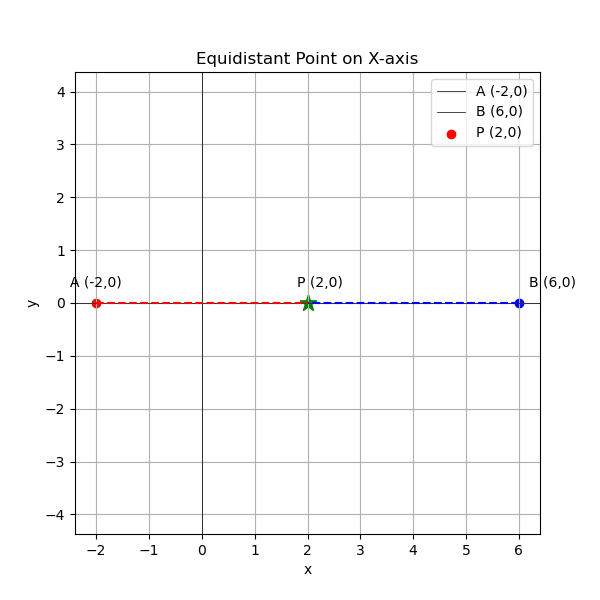
\includegraphics[width=\columnwidth, height=0.8\textheight, keepaspectratio]{figs/fig2.png}     
\end{frame}

\begin{frame}[fragile]
\frametitle{C Code}
\begin{lstlisting}
#include <stdio.h>
#include <math.h>

// Function to compute x-coordinate of equidistant point
double equidistant_point(double ax, double ay, double bx, double by) {
    // Norm squared of A and B
    double normA2 = ax*ax + ay*ay;
    double normB2 = bx*bx + by*by;

    double denom = 2 * (ax - bx);

    double x = (normA2 - normB2) / denom;
    return x;
}
\end{lstlisting}

\end{frame}

\begin{frame}[fragile]
\frametitle{Python and C Code}

\begin{lstlisting}
import ctypes
import matplotlib.pyplot as plt

lib = ctypes.CDLL("./libequidistant.so")
lib.compute_point.argtypes = [ctypes.c_double, ctypes.c_double,
                              ctypes.c_double, ctypes.c_double,
                              ctypes.POINTER(ctypes.c_double), ctypes.POINTER(ctypes.c_double)]

Ax, Ay = -2., 0.
Bx, By = 6., 0
\end{lstlisting}

\end{frame}
\begin{frame}[fragile]
\frametitle{Python and C Code}

\begin{lstlisting}
Px, Py = ctypes.c_double(), ctypes.c_double()

lib.compute_point(Ax, Ay, Bx, By, ctypes.byref(Px), ctypes.byref(Py))

Px_val, Py_val = Px.value, Py.value

print(f"A = ({Ax}, {Ay})")
print(f"B = ({Bx}, {By})")
print(f"Computed P = ({Px_val}, {Py_val})")
plt.figure()
plt.scatter([Ax, Bx, Px_val], [Ay, By, Py_val],
            color=["green", "red", "blue"], s=100)

\end{lstlisting}
\end{frame}

\begin{frame}[fragile]
\frametitle{Python and C Code}
\begin{lstlisting}
plt.text(Ax + 0.2, Ay, f"A({Ax:.2f},{Ay:.2f})", fontsize=12, color="green")
plt.text(Bx + 0.2, By, f"B({Bx:.2f},{By:.2f})", fontsize=12, color="red")
plt.text(Px_val + 0.2, Py_val, f"P({Px_val:.2f},{Py_val:.2f})", fontsize=12, color="blue")

plt.plot([Ax, Px_val, Bx], [Ay, Py_val, By],
         linestyle="--", color="gray")

plt.xlabel("X-axis")
plt.ylabel("Y-axis")
plt.title("Computed P = (A + B)/2")
plt.grid(True)
plt.axis("equal")
plt.savefig("fig2.1.png") 
plt.show()
\end{lstlisting}
\end{frame}


\begin{frame}{Plot-Using by both C and Python}
    \centering
    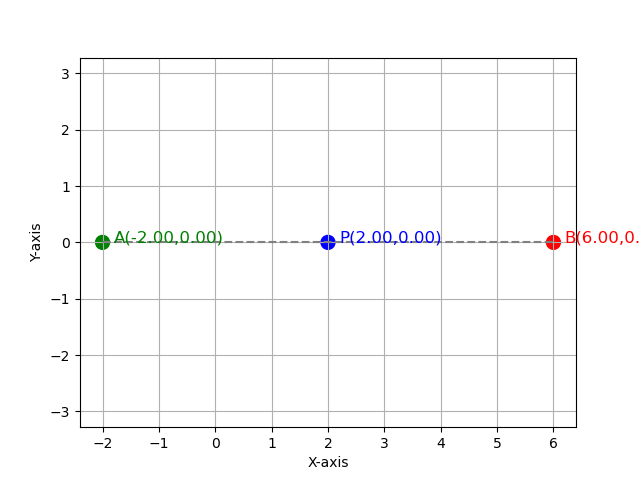
\includegraphics[width=\columnwidth, height=0.8\textheight, keepaspectratio]{figs/fig2.1.png}     
\end{frame}

\end{document}